% little trick to replace lib.tex by this
\renewcommand{\doctitle}[1]{
	\chapter{#1}
}
\renewcommand{\biblio}[1]{}
\doctitle{Le clavier}
Le clavier considéré ici comprend 12 touches, une pour
chaque note et sa dièse correspondante. Quatre autres
boutons permettent de passer d'une octave à une autre.
Le clavier permet de générer des fréquences allant de
\unit{523.25}{\hertz} à \unit{7902.1}{\hertz} et couvre
donc les octaves 5 à 8.

La figure \ref{fig:keyboard-circuit} représente le
circuit du clavier. Le clavier est composé de deux
réseaux de diviseurs résistifs. Le réseau constitué
des quatre potentiomètres permet de gérer les octaves
tandis que le réseau constitué des douze résistances
correspond aux notes et aux dièses correspondantes.

\begin{figure}[ht]
	\centering
	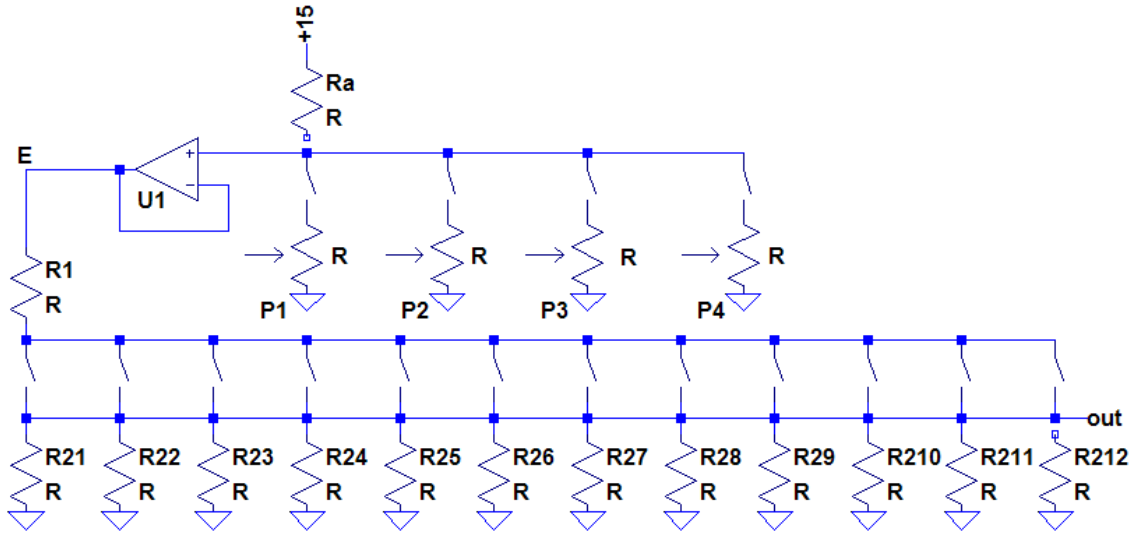
\includegraphics[scale=0.5]{img-keyboard/keyboard-circuit.png}
	\caption{Circuit du clavier.}
	\label{fig:keyboard-circuit}
\end{figure}

La tension étiquetée \textbf{out} sur la figure
\ref{fig:keyboard-circuit} sera appliquée à l'entrée
du VCO\footnote{Il est essentiel de prendre la tension à cet
endroit, et non avant les interrupteurs. Cela permet au clavier
de ne générer une tension non-nulle que quand une touche est pressée.},
qui produira ensuite à sa sortie un signal
périodique dont la fréquence est directement 
proportionnelle à l'entrée, selon la convention
\unit{1}{\milli\volt} correspond à \unit{1}{\hertz}. Cette
tension $\text{out}$ est donnée par la formule 
\[ \text{out} = E\frac{R_{2i}}{R_{2i} + R_1} \text{  avec  } i = 1\dots12. \]

Le dimensionnement complet du clavier se base
sur cette formule. En dimensionnant dans un premier
temps le clavier pour l'octave 8, l'obtention
de l'octave 7 est immédiate en divisant la tension
$E$ par deux, et ainsi de suite pour l'octave 6 et 5.
C'est précisément le rôle du réseau de diviseurs
résistifs constitué par les potentiomètres. L'utilisation
de potentiomètres à la place de simples résistances
permet de ``calibrer'' le circuit afin de conserver
une bonne précision (car en pratique l'alimentation
ne vaut pas exactement \unit{15}{\volt}).
Des valeurs de potentiomètres différentes sont utilisées
afin de permettre un calibrage plus simple.
Arbitrairement, $E$ vaut \unit{14}{\volt} pour l'octave
8 et est divisé par 2 pour chaque octave inférieure.

La présence d'un amplificateur suiveur entre ce premier
réseau de diviseurs résistifs et le suivant est indispensable
pour éviter les rendre indépendants.

Le tableau \ref{tab:keyboard-dim} résume les résultats du dimensionnement
du clavier. Seules les valeurs standard de la série de Renard
E12 ont été utilisées. En utilisant une combinaison de 3
résistances en séries ou en parallèles, une erreur inférieure
à 0.01\% est garantie (sans tenir compte des tolérances des
résistances). En utilisant une combinaison plus économique
de seulement 2 résistances, des erreurs bien plus grandes
peuvent survenir (de l'ordre de 0.10\% à 0.30\%). Une telle
erreur est encore raisonnable pour l'oreille humaine qui ne
peut pas différencier deux sons dont la fréquence ne diffère
pas de plus de 0.6\%\cite{frequency-jnd}. Cependant, ces erreurs
risquent encore d'être amplifiées dans les blocs suivant du
synthétiseur, il est donc préférable de les minimiser au maximum
dans ce premier bloc.

% TODO : a spliter en deux tableau (premier et deuxième réseau)
\begin{table}[ht]
	\centering
		\begin{tabular}{|c|c|}
			\hline
				Résistance & Valeur (en\unit{}{\kilo\ohm}) \\
			\hline
				$R_a$ & 0.47 \\
			\hline
				$P_1$ & maximum 10 \\
			\hline
				$P_2$ & maximum 1 \\
			\hline
				$P_3$ & maximum 0.47 \\
			\hline
				$P_4$ & maximum 0.1 \\
			\hline
		\end{tabular}
		\quad
		\begin{tabular}{|c|c|}
			\hline
				Résistance & Valeur (en\unit{}{\kilo\ohm}) \\
			\hline
				$R_1$ & 10 \\
			\hline
				$R_{21}$ & 82 | (15 + 0.390) \\
			\hline
				$R_{22}$ & 3.3 + (680 | 8.2) \\
			\hline
				$R_{23}$ & 10 + (0.120 | 2.7) \\
			\hline
				$R_{24}$ & 22 | (0.330 + 15) \\
			\hline
				$R_{25}$ & 15 | 1000 | 18 \\
			\hline
				$R_{26}$ & 100 | 220 | 8.2 \\
			\hline
				$R_{27}$ & 150 | (0.150 + 6.8) \\
			\hline
				$R_{28}$ & 8.2 | 39 | 56 \\
			\hline
				$R_{29}$ & 4.7 + (0.820 | 270) \\
			\hline
				$R_{210}$ & 220 | (0.470 + 4.7) \\
			\hline
				$R_{211}$ & 0.056 + (4.7 | 180) \\
			\hline
				$R_{212}$ & 2.7 + (1.8 | 12) \\
			\hline
		\end{tabular}
	\caption{Résumé du dimensionnement du clavier.}
	\label{tab:keyboard-dim}
\end{table}

Le tableau \ref{tab:keyboard-measure-vs-theory} donne quant
à lui les valeurs mesurées de la tension out. Les imprécisions
s'expliquent par les imprécisions des résistances et/ou du
calibrage.

\begin{table}[ht]
	\centering
		\begin{tabular}{|c|c|c|c|c|}
			\hline
				\specialcell{Octave $\rightarrow$ \\ Note $\downarrow$} & 5 & 6 & 7 & 8 \\
			\hline
				 C & \unit{510}{\milli\volt} (-2.53\%) & \unit{1040}{\milli\volt} (-0.62\%) & \unit{2100}{\milli\volt} (+0.33\%) & \unit{4160}{\milli\volt} (-0.86\%) \\
			\hline
				 C\# & \unit{547}{\milli\volt} (-1.26\%) & \unit{1100}{\milli\volt} (-0.78\%) & \unit{2230}{\milli\volt} (-0.58\%) & \unit{4460}{\milli\volt} (-0.565\%) \\
			\hline
				 D &  \unit{570}{\milli\volt} (-2.95\%) & \unit{1180}{\milli\volt} (+0.45\%) & \unit{2390}{\milli\volt} (+1.73\%) & \unit{4720}{\milli\volt} (+0.45\%) \\
			\hline
				 D\# & \unit{590}{\milli\volt} (-5.18\%) & \unit{1240}{\milli\volt} (-0.36\%) & \unit{2510}{\milli\volt} (+0.84\%) & \unit{4950}{\milli\volt} (-0.56\%) \\
			\hline
				 E & \unit{640}{\milli\volt} (-2.92\%) & \unit{1305}{\milli\volt} (-1.02\%) & \unit{2640}{\milli\volt} (+0.11\%) & \unit{5200}{\milli\volt} (-1.40\%) \\
			\hline
				 F & \unit{680}{\milli\volt} (-2.64\%) & \unit{1390}{\milli\volt} (-0.49\%) & \unit{2790}{\milli\volt} (-0.14\%) & \unit{5500}{\milli\volt} (-1.56\%) \\
			\hline
				 F\# & \unit{720}{\milli\volt} (-2.70\%) & \unit{1470}{\milli\volt} (-0.67\%) & \unit{2950}{\milli\volt} (-0.34\%) & \unit{5840}{\milli\volt} (-1.35\%) \\
			\hline
				 G & \unit{770}{\milli\volt} (-1.78\%) & \unit{1560}{\milli\volt} (-0.51\%) & \unit{3140}{\milli\volt} (+0.13\%) & \unit{6180}{\milli\volt} (-1.46\%) \\
			\hline
				 G\# & \unit{830}{\milli\volt} (-0.07\%)& \unit{1660}{\milli\volt} (-0.07\%) & \unit{3350}{\milli\volt} (+0.8\%) & \unit{6600}{\milli\volt} (-0.6\%) \\
			\hline
				 A & \unit{860}{\milli\volt} (-2.27\%) & \unit{1750}{\milli\volt} (-0.57\%) & \unit{3510}{\milli\volt} (-0.28\%) & \unit{6940}{\milli\volt} (-1.42\%) \\
			\hline
				 A\# & \unit{915}{\milli\volt} (-1.86\%) & \unit{1850}{\milli\volt} (-0.79\%) & \unit{3730}{\milli\volt} (+0.02\%) & \unit{7380}{\milli\volt} (-1.05\%) \\
			\hline
				 B & \unit{970}{\milli\volt} (-1.79\%) & \unit{1960}{\milli\volt} (-0.78\%) & \unit{3960}{\milli\volt} (+0.22\%) & \unit{7790}{\milli\volt} (-1.42\%) \\
			\hline
		\end{tabular}
	\caption{Résumé des mesures effectués avec erreur relative calculées par comparaison avec
	le tableau suivant \url{http://en.wikipedia.org/wiki/Scientific_pitch_notation\#Table_of_note_frequencies}. 
	Certaines lignes manquent car nous n'avions pas les bonnes résistances.}
	\label{tab:keyboard-measure-vs-theory}
\end{table}

Pour améliorer la précision du clavier, on peut :
\begin{itemize}
	\item Utiliser des potentiomètres à la place des combinaisons
	de résistances, et calibrer le clavier avant chaque utilisation.
	Cependant cette solution n'est ni économique (un potentiomètre
	coûte beaucoup plus cher qu'une résistance) ni pratique (nécessitera
	un long calibrage) ;
	\item Utiliser des résistances plus précises ($\pm$ 1\% par exemple) ;
	\item Mesurer chaque résistance utilisée et remplacer celles dont la
	valeur est trop imprécise par une autre plus précise.
\end{itemize}

\biblio{keyboard}

\end{document}